
The following is a curated list of the primary Julia commands that we use in ROB 101. The list is not meant to be exhaustive. You will want to add all of htese comamnds and more to your personal curated list of Julia commands; see Chapter~\ref{sec:GoogleDoc4Commands}.

\section{Creating Vectors and Matrices}
\label{sec:AppendixA:CreateVectorsMatrices}

Vectors and Matrices in Julia can hold variables of a single \texttt{Type}. We are primarily using
variables with these 4 types
\begin{enumerate}
        \renewcommand{\labelenumi}{(\alph{enumi})}
        \setlength{\itemsep}{.1cm}
    \item \texttt{Int64}
    \item \texttt{Float64}
    \item \texttt{Char}
    \item \texttt{String}
\end{enumerate}

\textbf{How to create vectors:}

\begin{enumerate}
        \renewcommand{\labelenumi}{(\alph{enumi})}
        \setlength{\itemsep}{.1cm}
    \item Separate elements by commas or semicolons:
    \begin{lstlisting}[language=Julia,style=mystyle]
animalsVector = ["lemur", "elephant", "tiger", "panda", "zebra", "cuttlefish"]
\end{lstlisting}
\textbf{Output} 
\begin{verbatim}
6-element Vector{String}:
 "lemur"
 "elephant"
 "tiger"
 "panda"
 "zebra"
 "cuttlefish"
\end{verbatim}

\begin{lstlisting}[language=Julia,style=mystyle]
numbersVector = numbersVector = [1; 2; 3; 4]
\end{lstlisting}
\textbf{Output} 
\begin{verbatim}
4-element Vector{Int64}:
 1
 2
 3
 4
\end{verbatim}

In lecture, we call the above a \textbf{column vector}.
  
    \item If you use spaces, then you obtain a $1 \times n$ matrix, which in lecture, we call a \textbf{row vector}
    \begin{lstlisting}[language=Julia,style=mystyle]
animalsVector = ["lemur" "elephant" "tiger" "panda" "zebra" "cuttlefish"]
\end{lstlisting}
\textbf{Output} 
\begin{verbatim}
1×6 Matrix{String}:
 "lemur"  "elephant"  "tiger"  "panda"  "zebra"  "cuttlefish"
\end{verbatim}

\begin{lstlisting}[language=Julia,style=mystyle]
numbersVector = [1.0 2 3 4]
\end{lstlisting}
\textbf{Output} 
\begin{verbatim}
1×4 Matrix{Float64}:
 1.0  2.0  3.0  4.0
\end{verbatim}

\item The infamous \textcolor{red}{\bf adjoint vector} is a special kind of row vector that when multiplied by a column vector of the appropriate size, produces a number and not a 1-element vector. 

\begin{lstlisting}[language=Julia,style=mystyle]
numbersVector = [1.0; 2; 3; 4]'
\end{lstlisting}
\textbf{Output} 
\begin{verbatim}
1×4 adjoint(::Vector{Float64}) with eltype Float64:
 1.0  2.0  3.0  4.0
\end{verbatim}

\begin{lstlisting}[language=Julia,style=mystyle]
x = [1; 2; 3.0]
y = [4; 5; 6]

@show x'  # adjoint of x, looks like a row vector

z=x'*y
\end{lstlisting}
\textbf{Output} 
\begin{verbatim}
x' = [1.0 2.0 3.0]

32.0
\end{verbatim}

\item \texttt{Vector\{Float64\}(undef, n)} creates an $n$-element vector with undefined entries. 

\item \texttt{Vector\{Float64\}(undef, 0)} creates a $0$-element vector with undefined entries. This is a truly empty vector.

\item If \texttt{A} is a \texttt{Vector}, then \texttt{B = copy(A)} creates the independent \texttt{Vector} \texttt{B} and it is a copy of the \texttt{Vector} \texttt{A}.

\item If \texttt{A} is a \texttt{Vector}, then \texttt{B = A} creates the \texttt{Vector} \texttt{B} and links it to $A$. Hence, changes to \texttt{A} also show up in \texttt{B} and vice versa, changes to \texttt{B} also show up in \texttt{A}. Usually, you do not want this to happen and hence you should consider the \texttt{copy} command. 


\end{enumerate}

\textbf{How to create matrices:}

\begin{enumerate}
        \renewcommand{\labelenumi}{(\alph{enumi})}
        \setlength{\itemsep}{.1cm}
    \item Use spaces to separate elements in a same row, and use either commas or semicolons to separate rows.
    \begin{lstlisting}[language=Julia,style=mystyle]
A=[1.0 2.0; 3.0 4.0]
\end{lstlisting}
\textbf{Output} 
\begin{verbatim}
2×2 Matrix{Float64}:
 1.0  2.0
 3.0  4.0
\end{verbatim}

\item \texttt{zeros}(n,m)
\item \texttt{ones}(n,m)
\item \texttt{using Random}
\item \texttt{Random.seed!(4321)} or whatever value you want sets the ``seed'' of the random number generators. This way, we can get repeatable results in HW.
\item  \texttt{rand}(n,m) (uniform) and with an extra ``n'' \texttt{randn}(n,m) (normal, aka Gaussian or Bell Curve)
\item There is no explicit command to create an $n \times n$ identity matrix. You do it like so
\begin{lstlisting}[language=Julia,style=mystyle]
# how to make an identity matrix in Julia
using LinearAlgebra
n=4 # set your size here
Id = zeros(n,n) + I
# I is a special operator that when added to a square zero martrix 
# produces an identity matrix of the appropriate size
\end{lstlisting}
\textbf{Output} 
\begin{verbatim}
4×4 Matrix{Float64}:
 1.0  0.0  0.0  0.0
 0.0  1.0  0.0  0.0
 0.0  0.0  1.0  0.0
 0.0  0.0  0.0  1.0
\end{verbatim}

The operator \texttt{I} is part of the \texttt{LinearAlgebra} package. If you have not already called \texttt{using LinearAlgebra}, you will not be able to use the identity operator \texttt{I}. 

\item  \texttt{Matrix\{Float64\}(undef, n, m)} creates a matrix of a specified size without specifying its entries. Note that \texttt{undef} is a Julia keyword to create a value that is ``undefined''.\\

\begin{lstlisting}[language=Julia,style=mystyle]
Matrix{Float64}(undef, 3, 4)
\end{lstlisting}
\textbf{Output} 
\begin{verbatim}
3×4 Matrix{Float64}:
 6.90947e-310  6.90947e-310  6.90947e-310  6.90947e-310
 6.90947e-310  6.90947e-310  6.90947e-310  6.9094e-310
 6.90947e-310  6.90947e-310  6.90947e-310  6.90947e-310
\end{verbatim}

\item  \texttt{Matrix\{Float64\}(undef, n, 0)} creates a matrix with n rows and zero columns, while to create a matrix with zero rows and m columns, you use the command \texttt{Matrix\{Float64\}(undef, 0, m)}.


\end{enumerate}


\section{Indexing or Slicing Vectors and Matrices}
\label{sec:AppendixA:Indexing}

\begin{rem}
\textcolor{red}{\bf Julia uses **1-based indexing** which means that the index starts at 1 and not 0.} Be aware that 0-based indexing is used in some other programming languages, such as C++. If you are familiar with MATLAB, it uses 1-based indexing.
\end{rem}


\begin{lstlisting}[language=Julia,style=mystyle]
@show row_vec = [1 3 5 7 9]
println(" ")
# Indexing one or more elements 
@show x=row_vec[3]
@show x=row_vec[2:3]
@show x=row_vec[2:end]
@show x=row_vec[[2 3 5]]
\end{lstlisting}
\textbf{Output} 
\begin{verbatim}
row_vec = [1 3 5 7 9] = [1 3 5 7 9]
 
x = row_vec[3] = 5
x = row_vec[2:3] = [3, 5]
x = row_vec[2:end] = [3, 5, 7, 9]
x = row_vec[[2 3 5]] = [3 5 9]

1×3 Matrix{Int64}:
 3  5  9
\end{verbatim}

\begin{lstlisting}[language=Julia,style=mystyle]
using Random # Using an external pacakge called Random 
Random.seed!(1234) # Set the seed so that each of you get the same results. 
A = rand(4, 6)

x = A[:,2]
\end{lstlisting}
\textbf{Output} 
\begin{verbatim}
4-element Vector{Float64}:
 0.7940257103317943
 0.8541465903790502
 0.20058603493384108
 0.2986142783434118
\end{verbatim}

\begin{lstlisting}[language=Julia,style=mystyle]
using Random # Using an external pacakge called Random 
Random.seed!(1234) # Set the seed so that each of you get the same results. 
A = rand(4, 6)

x = A[2,:] # Produces a column vector!
\end{lstlisting}
\textbf{Output} 
\begin{verbatim}
6-element Vector{Float64}:
 0.7667970365022592
 0.8541465903790502
 0.5796722333690416
 0.9567533636029237
 0.6516642063795697
 0.9646697763820897
\end{verbatim}

\begin{lstlisting}[language=Julia,style=mystyle]
using Random # Using an external pacakge called Random 
Random.seed!(1234) # Set the seed so that each of you get the same results. 
A = rand(4, 6)

x = A[2:2,:] # to keep it as a row
\end{lstlisting}
\textbf{Output} 
\begin{verbatim}
1×6 Matrix{Float64}:
 0.766797  0.854147  0.579672  0.956753  0.651664  0.96467
\end{verbatim}

\begin{lstlisting}[language=Julia,style=mystyle]
using Random # Using an external pacakge called Random 
Random.seed!(1234) # Set the seed so that each of you get the same results. 
A = rand(4, 6)

x = A[3:end,3:end]
\end{lstlisting}
\textbf{Output} 
\begin{verbatim}
2×4 Matrix{Float64}:
 0.648882   0.646691  0.0566425  0.945775
 0.0109059  0.112486  0.842714   0.789904
\end{verbatim}

\begin{lstlisting}[language=Julia,style=mystyle]
using Random # Using an external pacakge called Random 
Random.seed!(1234) # Set the seed so that each of you get the same results. 
A = rand(4, 6)
#
indRow = [3, 4]  # note the commas
indCol = [2, 5, 6] # note the commas
#
x = A[indRow,indCol]
\end{lstlisting}
\textbf{Output} 
\begin{verbatim}
2×3 Matrix{Float64}:
 0.200586  0.0566425  0.945775
 0.298614  0.842714   0.789904
\end{verbatim}

\section{1-Element Vectors and 1 x 1 Matrices}
\label{sec:AppendixA:1ElementVectors}

A $ 1 \times n$ matrix times an $ n \times 1$ vector produces a 1-element vector in Julia. You have to extract the element from the vector if you want to use it for assigning an element some other vector or matrix.

\begin{lstlisting}[language=Julia,style=mystyle]
A = [1.0  2]
b = [2.0; 3.0]
y=A*b 
\end{lstlisting}
\textbf{Output} 
\begin{verbatim}
1-element Vector{Float64}:
 8.0
\end{verbatim}

Note that $y$ is a 1-element vector. \\

\begin{lstlisting}[language=Julia,style=mystyle]
@show y
@show y[1]
\end{lstlisting}
\textbf{Output} 
\begin{verbatim}
y = [8.0]
y[1] = 8.0

8.0
\end{verbatim}


\begin{lstlisting}[language=Julia,style=mystyle]
A=zeros(2,3)
A[1,3] = y
\end{lstlisting}
\textbf{Output} 
\begin{verbatim}
MethodError: Cannot `convert` an object of type Vector{Float64} to an object of type
Float64
Closest candidates are:
  convert(::Type{T}, ::T) where T<:Number at number.jl:6
  convert(::Type{T}, ::Number) where T<:Number at number.jl:7
  convert(::Type{T}, ::Base.TwicePrecision) where T<:Number at twiceprecision.jl:250
  ...

Stacktrace:
 [1] setindex!(::Matrix{Float64}, ::Vector{Float64}, ::Int64, ::Int64)
   @ Base ./array.jl:841
 [2] top-level scope
   @ In[34]:2
 [3] eval
   @ ./boot.jl:360 [inlined]
 [4] include_string(mapexpr::typeof(REPL.softscope), mod::Module, code::String, filename::String)
   @ Base ./loading.jl:1094
\end{verbatim}

\begin{lstlisting}[language=Julia,style=mystyle]
A=zeros(2,3)
A[1,3] = y[1]
A
\end{lstlisting}
\textbf{Output} 
\begin{verbatim}
2×3 Matrix{Float64}:
 0.0  0.0  8.0
 0.0  0.0  0.0
\end{verbatim}

The product of a $1 \times n$ adjoint vector and an $n$-element vector is a scalar and not some kind of array. You do not need to extract the final answer in order to use it somewhere at a later point. In the output, note that there are no brackets around the number $8.0$ or other indication that the result is a vector.\\
 
\begin{lstlisting}[language=Julia,style=mystyle]
x = [1.0;  2]
y = [2.0; 3.0]
@show x'
@show y
z=x'*y
\end{lstlisting}
\textbf{Output} 
\begin{verbatim}
x' = [1.0 2.0]
y = [2.0, 3.0]

8.0
\end{verbatim}

Where as here we multiply a $1 \times 2$ matrix times a $2 \times 1$ vector in Julia and produce a 1-element vector.

\begin{lstlisting}[language=Julia,style=mystyle]
x = [1.0  2]
y = [2.0; 3.0]
@show x
@show y
z=x*y
\end{lstlisting}
\textbf{Output} 
\begin{verbatim}
x = [1.0 2.0]
y = [2.0, 3.0]

1-element Vector{Float64}:
 8.0
\end{verbatim}

\section{Size vs Length Commands, Which to use for Vectors and Matrices}

\begin{lstlisting}[language=Julia,style=mystyle]
A = [ 1 2 3; 4 5 6; 7 8 9]
\end{lstlisting}
\textbf{Output} 
\begin{verbatim}
3×3 Matrix{Int64}:
 1  2  3
 4  5  6
 7  8  9
\end{verbatim}

\begin{lstlisting}[language=Julia,style=mystyle]
b=[1;2;3]
\end{lstlisting}
\textbf{Output} 
\begin{verbatim}
3-element Vector{Int64}:
 1
 2
 3
\end{verbatim}

\begin{lstlisting}[language=Julia,style=mystyle]
length(b)
\end{lstlisting}
\textbf{Output} 
\begin{verbatim}
3
\end{verbatim}

\begin{lstlisting}[language=Julia,style=mystyle]
length(A) # gives total number of elements in A
\end{lstlisting}
\textbf{Output} 
\begin{verbatim}
9
\end{verbatim}

\begin{lstlisting}[language=Julia,style=mystyle]
size(A) # number of rows and number of columns
\end{lstlisting}
\textbf{Output} 
\begin{verbatim}
(3, 3)
\end{verbatim}

\begin{lstlisting}[language=Julia,style=mystyle]
nRowsA, nColsA = size(A) # number of rows and number of columns 
@show nRowsA
nColsA
\end{lstlisting}
\textbf{Output} 
\begin{verbatim}
nRowsA = 3

3
\end{verbatim}

It is not recommended to apply the \texttt{size} command to a \texttt{Vector}, but it does return an answer.

\begin{lstlisting}[language=Julia,style=mystyle]
size(b)
\end{lstlisting}
\textbf{Output} 
\begin{verbatim}
(3,)
\end{verbatim}

If you try to assign the number of columns, you'll get an error, however. It really is better not to use the \texttt{size} command on vectors.

\begin{lstlisting}[language=Julia,style=mystyle]
nRowsb, nColsb = size(b)
\end{lstlisting}
\textbf{Output} 
\begin{verbatim}
BoundsError: attempt to access Tuple{Int64} at index [2]

Stacktrace:
 [1] indexed_iterate(t::Tuple{Int64}, i::Int64, state::Int64)
   @ Base ./tuple.jl:86
 [2] top-level scope
   @ In[11]:1
 [3] eval
   @ ./boot.jl:360 [inlined]
 [4] include_string(mapexpr::typeof(REPL.softscope), mod::Module, code::String, filename::String)
   @ Base ./loading.jl:1094

\end{verbatim}

You can also obtain the number of rows or just the number of columns of a matrix.

\begin{lstlisting}[language=Julia,style=mystyle]
A=rand(3,4)
display(A)
@show nRows = size(A,1); # note the 1
\end{lstlisting}
\textbf{Output} 
\begin{verbatim}
3×4 Matrix{Float64}:
 0.658815  0.59552   0.61816   0.0368842
 0.515627  0.292462  0.66426   0.643704
 0.260715  0.28858   0.753508  0.
 
nRows = size(A, 1) = 3
\end{verbatim}

\begin{lstlisting}[language=Julia,style=mystyle]
A=rand(3,4)
display(A)
@show nCols = size(A,2);  # note the 2
\end{lstlisting}
\textbf{Output} 
\begin{verbatim}
3×4 Matrix{Float64}:
 0.525057  0.082207  0.218177  0.932984
 0.61201   0.199058  0.362036  0.827263
 0.432577  0.576082  0.204728  0.0992992
 
nCols = size(A, 2) = 4
\end{verbatim}

\vspace*{.2cm}

\begin{tcolorbox}[title = {\bf \large Length vs Size}]

\begin{itemize}
    \item \texttt{length(X)} is the total number of elements in the array $X$. If $X$ is a vector, then it is the usual length. If $X$ is a matrix, then length returns the product of the number of rows and the number of columns.
    
    \item \texttt{nRows, nCols = size(A)} is best applied to matrices. It provides the number of rows and the number of columns. You can also use it as follows to return just the number of rows or just the number of columns,
    
    \item \texttt{nRows = size(A,1)}
    
  \item \texttt{nCols = size(A,2)} 
  
  \item Applying the \texttt{size} command to vectors is just asking for trouble. Please avoid doing this.
\end{itemize}


\end{tcolorbox}


\section{Flow Control: If-then-else and Looping}
\label{sec:AppendixA:FlowControl}

\begin{lstlisting}[language=Julia,style=mystyle]
# Read me and run me
# More conditions can be evaluated using elseif
x = 1
y = 1
if x < y
    println("x is less than y")
elseif x > y
    println("x is greater than y")
else
    println("x is equal to y")
end
\end{lstlisting}
\textbf{Output} 
\begin{verbatim}
x is equal to y
\end{verbatim}



\begin{lstlisting}[language=Julia,style=mystyle]
x=[4.0]
if length(x) == 1
    if string(typeof(x))[1:6] == "Vector" # Double equals means EQUIVALENT TO
        @show typeof(x)
        @show typeof(x[1])
        @show x=x[1]
    else
        @show x
    end
end
x
\end{lstlisting}
\textbf{Output} 
\begin{verbatim}
typeof(x) = Vector{Float64}
typeof(x[1]) = Float64
x = x[1] = 4.0

4.0
\end{verbatim}

\begin{lstlisting}[language=Julia,style=mystyle]
# Run me to see the counter augment by 2 as we go through the loop
mySum=0
for k = 13:2:26 #k_start:k_increment:k_end note the extra colon
    mySum = mySum + k # add k to mySum
    @show (k, mySum)
end
mySum
\end{lstlisting}
\textbf{Output} 
\begin{verbatim}
(k, mySum) = (13, 13)
(k, mySum) = (15, 28)
(k, mySum) = (17, 45)
(k, mySum) = (19, 64)
(k, mySum) = (21, 85)
(k, mySum) = (23, 108)
(k, mySum) = (25, 133)

133
\end{verbatim}


\begin{lstlisting}[language=Julia,style=mystyle]
A=[
-0.991273  -0.850184  -1.06297    0.609128   0.498376   0.411742
 -0.0        0.592798  -0.509626  -0.547334  -0.670348  -0.826093
  0.0       -0.0        0.673963   0.24726   -0.52135    0.680463
 -0.0       -0.0        0.0       -0.860824  -0.71363   -0.322208
 -0.0        0.0       -0.0        0.0        0.249046   0.373825
  0.0       -0.0       -0.0        0.0        0.0       -0.044526
]
#
b=[0.6849753810315695
 0.7387064229251636
 0.8252920694637993
 0.2707345660171885
 0.254653180382145
 0.1555903546558295]; #semicolon suppresses output

\end{lstlisting}
\textbf{Output} 
\begin{verbatim}
(nothing)
\end{verbatim}

\begin{lstlisting}[language=Julia,style=mystyle]
N=length(b)
x=zeros(N,1) # Makes x an N x 1 matrix of zeros
x[N] = b[N]/A[N,N]
for i = (N-1):-1:1
    x[i] = (b[i]-A[i,i+1:end]'*x[i+1:end])/A[i,i]
end
x
\end{lstlisting}
\textbf{Output} 
\begin{verbatim}
6×1 Matrix{Float64}:
 -21.381592956092216
   9.163388707678338
  11.142804824616672
  -4.202499623521532
   6.267662793927989
  -3.494370809321059
\end{verbatim}

A second kind of loop, the \texttt{while\,loop}.

\begin{lstlisting}[language=Julia,style=mystyle]
N=277777788888899
i=0; Ndigits=digits(N);K=length(Ndigits)  
while (K>1)
    i=i+1    
    prodN=Ndigits[1]
    for k = 2:K
       prodN=prodN*Ndigits[k]
    end
    @show prodN
    Ndigits=digits(prodN)
    K=length(Ndigits)  
end
println("The multiplicative persistence of $N is  $i")
\end{lstlisting}
\textbf{Output} 
\begin{verbatim}
prodN = 4996238671872
prodN = 438939648
prodN = 4478976
prodN = 338688
prodN = 27648
prodN = 2688
prodN = 768
prodN = 336
prodN = 54
prodN = 20
prodN = 0
The multiplicative persistence of 277777788888899 is  11
\end{verbatim}



\section{Functions}
\label{sec:AppendixA:Functions}
\begin{lstlisting}[language=Julia,style=mystyle]
# Simplest kind of function
f(x) = 5x + 2
\end{lstlisting}
\textbf{Output} 
\begin{verbatim}
f (generic function with 1 method)
\end{verbatim}

\begin{lstlisting}[language=Julia,style=mystyle]
f(x) = x + 4*x + sin(x)*x
\end{lstlisting}
\textbf{Output} 
\begin{verbatim}
f (generic function with 1 method)
\end{verbatim}

\begin{lstlisting}[language=Julia,style=mystyle]
f(pi/4)
\end{lstlisting}
\textbf{Output} 
\begin{verbatim}
4.482351184257038
\end{verbatim}

\begin{lstlisting}[language=Julia,style=mystyle]
function f(x)
    y = x + 4*x + sin(x)*x
    return y
end
\end{lstlisting}
\textbf{Output} 
\begin{verbatim}
f (generic function with 1 method)
\end{verbatim}

\begin{lstlisting}[language=Julia,style=mystyle]
f(pi/4)
\end{lstlisting}
\textbf{Output} 
\begin{verbatim}
4.482351184257038
\end{verbatim}

\begin{lstlisting}[language=Julia,style=mystyle]
function peel_one_layer(Temp, k)
    pivot = Temp[k, k]
    if abs(pivot) < 1e-6
        C=NaN;R=NaN;Temp=NaN
        println("Pivot is too small")
    else
        C = Temp[:, k] / pivot
        R = Temp[k:k, :]
        Temp = Temp - C*R
    end
    return C, R, Temp
end
\end{lstlisting}
\textbf{Output} 
\begin{verbatim}
peel_one_layer (generic function with 1 method)
\end{verbatim}

\begin{lstlisting}[language=Julia,style=mystyle]
function myLU(A)
    Temp = copy(A) # Initialize Temp matrix by 
                #copying the original matrix A
    nRows, nCols = size(Temp) # Get the size of the input matrix
    K = minimum([nRows, nCols])
    # Initialize the lower and upper triangular matrix
    L = zeros(Float64, (nRows, K)) # Using zeros function by
                                # specifying both type and size
    U = zeros(Float64, (K, nCols)) 
    # Here we do the actual factorization
    for k = 1:K
        C, R, Temp = peel_one_layer(Temp, k) # calling a separate function
        L[:, k] = C
        U[k:k, :] = R
    end
    return L, U
end
\end{lstlisting}
\textbf{Output} 
\begin{verbatim}
myLU (generic function with 1 method)
\end{verbatim}

\begin{lstlisting}[language=Julia,style=mystyle]
using Random
using LinearAlgebra
Random.seed!(09182022)
A = randn(5, 7)
#
L, U = myLU(A)
\end{lstlisting}
\textbf{Output} 
\begin{verbatim}
([1.0 -0.0 … 0.0 -0.0; 1.3841751352784288 1.0 … 0.0 -0.0; … ; 1.8240441684383097 
1.7669720431792901 … 1.0 -0.0; 1.1660675070497575 0.4629237529415664 … 
-0.8475551711339656 1.0], [-0.3236905701556438 0.9372755784538437 … 
-0.009357226530146447 -0.0076384514441543774; 0.0 -2.1005108102249452 …
1.4460922800584077 0.41893233388727713; … ; 0.0 0.0 … 0.19792290864355966 
-0.6285612979102336; -5.551115123125783e-17 0.0 … -1.3304631421106152 
1.0052145594104471])
\end{verbatim}

\section{Applying Functions to Arrays via Broadcasting}

Julia has a special syntax for applying functions to individual elements of arrays. You need to add a ``dot'' after the function and before the argument to the function. It's best understood by doing it. 

\begin{lstlisting}[language=Julia,style=mystyle]
x = [0 pi/4 pi/2 3pi/4 pi 5pi/4]
\end{lstlisting}
\textbf{Output} 
\begin{verbatim}
1×6 Matrix{Float64}:
 0.0  0.785398  1.5708  2.35619  3.14159  3.92699
\end{verbatim}

\begin{lstlisting}[language=Julia,style=mystyle]
sin.(x)  # note the dot
\end{lstlisting}
\textbf{Output} 
\begin{verbatim}
1×6 Matrix{Float64}:
 0.0  0.707107  1.0  0.707107  1.22465e-16  -0.707107
\end{verbatim}

This also works with functions that you write yourself! It pretty awesome.

\begin{lstlisting}[language=Julia,style=mystyle]
f(x) = 1 + 2x + sin(x^2)
\end{lstlisting}
\textbf{Output} 
\begin{verbatim}
f (generic function with 1 method)
\end{verbatim}

\begin{lstlisting}[language=Julia,style=mystyle]
f.(x)  # note the dot
\end{lstlisting}
\textbf{Output} 
\begin{verbatim}
1×6 Matrix{Float64}:
 1.0  3.14927  4.76586  5.04438  6.85288  9.13678
\end{verbatim}



\section{Plotting}


\begin{lstlisting}[language=Julia,style=mystyle]
using Plots
gr()
time = 0:0.01:1
 x = exp.(time)
plot(time, x)
\end{lstlisting}
\textbf{Output} 
	\begin{center}
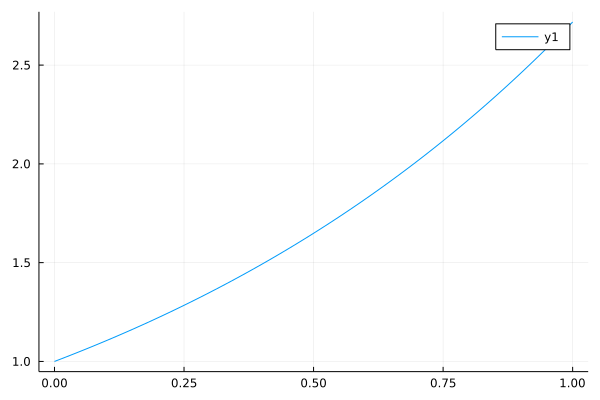
\includegraphics[width=0.5\columnwidth]{graphics/AppA/AppendixA_SimplePlot.png}
\end{center}


\begin{lstlisting}[language=Julia,style=mystyle]
time = 0:0.01:1
 x = exp.(time)
titre = "My Second Plot" 
plot(time, x, title=titre, linewidth=3, legend = false)
plot!(xlabel = "time (seconds)", ylabel = "x  (meters)")
\end{lstlisting}
\textbf{Output} 
\begin{center}
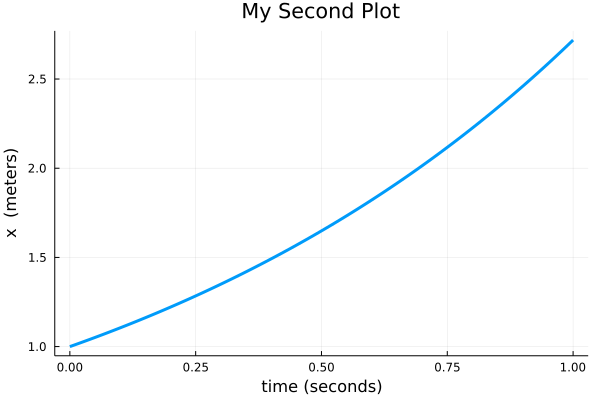
\includegraphics[width=0.5\columnwidth]{graphics/AppA/AppendixA_BetterPlot.png}
\end{center}

Recall that \texttt{\bf plot!} adds to the previous plot; the command is pronounced `` plot bang''.

\begin{lstlisting}[language=Julia,style=mystyle]
f(x) = .1x^3 + 2
g(x) = (x^2)*sin(3*x) 
xmin = -2*pi
xmax = 2*pi
titre = "My Third Plot"
plot(f, xmin,xmax, title=titre, linewidth=3) 
plot!(g, xmin,xmax, title=titre, linewidth=3)
plot!(xlabel = "x", ylabel = "y") 
\end{lstlisting}
\textbf{Output} 
\begin{center}
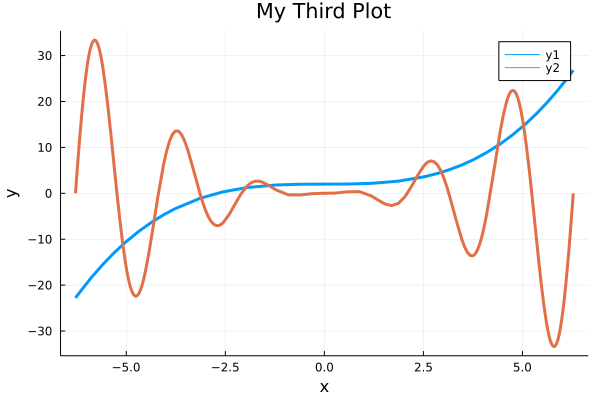
\includegraphics[width=0.5\columnwidth]{graphics/AppA/AppendixA_ThirdPlot.png}
\end{center}

\begin{lstlisting}[language=Julia,style=mystyle]
time = 0:0.01:1
 x = exp.(time)
plot(time, x)
png("AppendixA_SimplePlot") # Produces the png file
\end{lstlisting}
\textbf{Output} 
\begin{verbatim}
(nothing comes to the screen) You will find a .png file in your files tab. 

Select it and then hit the download button.
\end{verbatim}

% \begin{lstlisting}[language=Julia,style=mystyle]

% \end{lstlisting}
% \textbf{Output} 
% \begin{verbatim}

% \end{verbatim}

% \begin{lstlisting}[language=Julia,style=mystyle]

% \end{lstlisting}
% \textbf{Output} 
% \begin{verbatim}

% \end{verbatim}

% \begin{lstlisting}[language=Julia,style=mystyle]

% \end{lstlisting}
% \textbf{Output} 
% \begin{verbatim}

% \end{verbatim}
\section{Suggested Resources}

\begin{itemize}
\item Why Julia? \\ \url{https://juliadatascience.io/julia_accomplish}
    \item Why Julia in the eyes of MIT? \\ \url{https://web.mit.edu/18.06/www/Spring17/Julia-intro.pdf}
    \item Compares Matlab, Python, and Julia side by side\\ \url{https://cheatsheets.quantecon.org/}
    \item Noteworthy differences with Matlab \\ \url{https://docs.julialang.org/en/v1/manual/noteworthy-differences/}
    \item Rich source of plotting examples \\ \url{https://gist.github.com/gizmaa/7214002}
    \item Compact cheatsheet for plotting in Julia\\ \url{https://github.com/sswatson/cheatsheets/blob/master/plotsjl-cheatsheet.pdf}
    \item Very compact, maybe not the first resource you turn to \\ \url{https://juliadocs.github.io/Julia-Cheat-Sheet/}
    \item Julia for Data Science \\ \url{https://juliadatascience.io/}
\end{itemize}